% Indicate the main file. Must go at the beginning of the file.
% !TEX root = ../main.tex

%%%%%%%%%%%%%%%%%%%%%%%%%%%%%%%%%%%%%%%%%%%%%%%%%%%%%%%%%%%%%%%%%%%%%%%%%%%%%%%%
% 03_methods
%%%%%%%%%%%%%%%%%%%%%%%%%%%%%%%%%%%%%%%%%%%%%%%%%%%%%%%%%%%%%%%%%%%%%%%%%%%%%%%%

\section{Methods}
\label{methods}

    \subsection{Dataset}

    As part of the Wildlife@Campus project, a labeled dataset was created to train a deep learning algorithm.
    The dataset is divided into seven sessions.
    The sessions are an indication of the project stage where the data was added to the dataset.
    The images are grouped into sequences, each representing a sightin of an animal.
    The sequences are not standardized in length and range from 1 to 915 images per sequence.
    It is worth noting that in future use cases, the sequence length will likely be more standardized.
    The actual length will depend on the camera settings -- common settings such as 1, 3, 5, or 10 images per trigger -- which can be extracted from the EXIF information of the images.
    The dataset provides two types of labels -- the first one is not standardized and can vary between the sessions.
    For example scientific names and common names are used interchangeably, and there are different spellings.
    The second type is a simplified and standardized version with some visually not distinguishable species grouped together.
    For this project, only the simplified labels will be used.
    The distribution of available sequences per label is shown in \autoref{fig:sequenceperlabel}.
    The category \texttt{other} represents sequences containing more than one species, and the category \texttt{NaN} represents sequences without a label -- both will be excluded from the from the dataset.
    The category \texttt{glis\_glis} is represented in only four sequences, which is simply not enough to actually train the model to detect it.
    For this reason, it will be excluded from the dataset as well.
    20\% of the sequences will be set aside for testing.
    A stratified split with a fixed seed will be used to ensure reproducibility.

    \begin{figure}[ht]
    \centering
    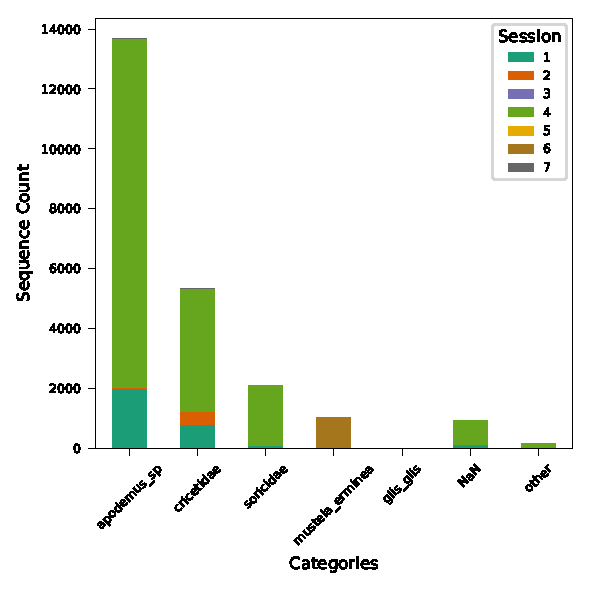
\includegraphics{figures/label2_session.pdf}
    \caption{Available sequences per label colored by session.}
    \label{fig:sequenceperlabel}
    \end{figure}


    \subsection{Processing}

    The processing of the images is divided into two main steps: 
    In a first step a detector is applied to identify the regions of interest (ROI) in the images, and to select which images are actually used for training.
    In a second step, the ROIs are processed to feed them into the model.

        \subsubsection{Detection and Selection}

        The Microsoft MegaDetector (MD) is a well-established model for detecting animals in camera trap images \autocite{hernandezPytorchWildlifeCollaborativeDeep2024a, velezChoosingAppropriatePlatform2022, schneiderRecognitionEuropeanMammals2024}.
        In this project, MD will be used to detect animals in all images of each sequence.
        An example of how this detections look like is shown in \autoref{fig:detection_example}.
        MD outputs a list of bounding boxes for detected animals, humans, and vehicles along with corresponding confidence scores. 
        All animal bounding boxes with a confidence score above a threshold of 0.5 will be extracted and used for classification.
        The images lost due to the detection process are shown in \autoref{fig:lost_images}.
        These n images or rather areas of images will be resized to a fixed size, working for the model used for feature extraction. 
        For training, the data will be augmented using random rotation and random flipping -- arguably the simplest augmentation techniques for images. 
        This is a common approach to increase the variety of the training data and improve the model's generalization \autocite{shortenSurveyImageData2019}.

        Prior to feeding the images into the model, the relevant areas are detected utilizing the Megadetector (MD) \autocite{morrisEfficientPipelineCamera2025}. 
        This tool is used to identify regions of interest (ROI) for each image, providing bounding boxes (BBox) with corresponding labels and confidence scores.
        From the provided labels -- \textit{animal}, \textit{human} and \textit{vehicle} -- only the \textit{animal} label is retained.
        This detection is performed on the original images for the whole dataset and storred as a json file per sequence for easy access during training.
        For the training only the BBox with the highest confidence score per image is selected and there is a minimal confidence score to actually concider an image was set to 0.5.

        \begin{figure}[ht]
        \centering
        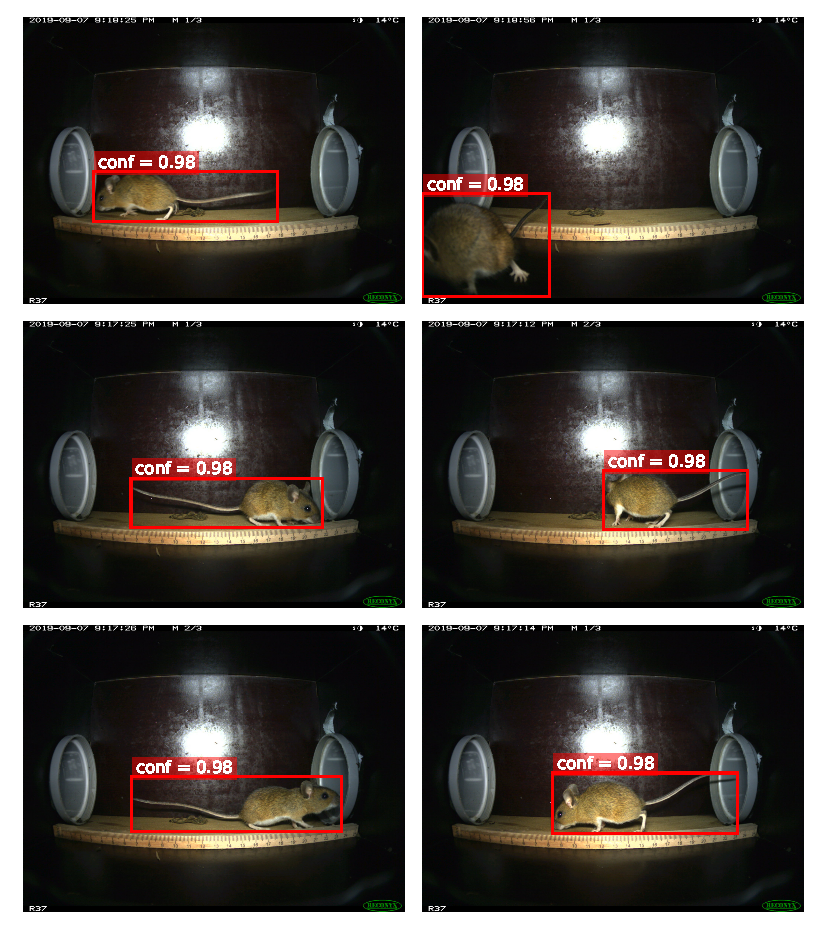
\includegraphics{figures/detections_on_a_sequence.pdf}
        \caption{Example of how the detections look like. The bounding boxes are the highest confidence detections for the sequence 1001824 a sample from the \textit{apodemus\_sp} category.}
        \label{fig:detection_example}
        \end{figure}

        \begin{figure}[ht]
        \centering
        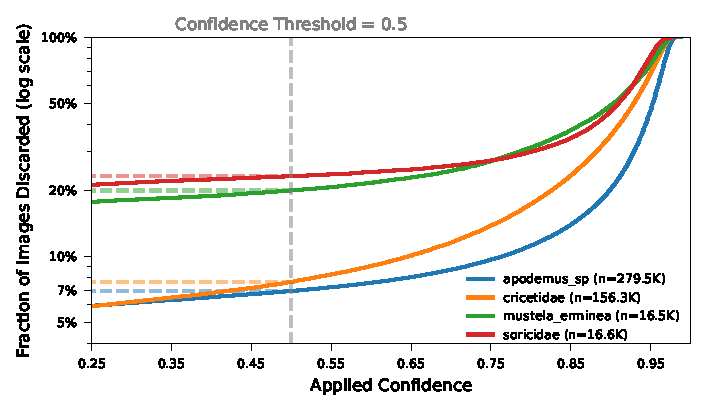
\includegraphics{figures/discarded_img_by_conf.pdf}
        \caption{Fraction of images lost per category for a detection confidence threshold of 0.5.}
        \label{fig:lost_images}
        \end{figure}

        \subsubsection{Image Preprocessing}
        To process the images a custom transformation pipline was implemented using transform version 2 from the torchvision library and a custom crop function.
        Cropping was done using the BBoxes from the MD detection extending the BBox in order to cut the ratio expected by the model applied.
        In the case that the extended BBox surpasses the image border the image is padded with black pixels.
        After cropping the image is resized to the expected input size of the model.
        The images are then converted to a tensor and normalized using the mean and standard deviation calculated on the dataset itself.
        To calculate mean and standard deviation the whole dataset was used since it is quite resource intensive to calculate and the same values are used for all folds.
        To create the most accurate mean and standard deviation for the actual model input only the best BBox area per image is used.
        Data augmentation was implemented and considered as an option but not actually used in the end.

    \subsection{Model}
    - how the models where adapted for the task (tool to detect type of last layer and rebuild it to fit the num classes)

    \subsection{Training Pipeline}
    - description of the training pipline using the PyTorch Lightning framework

    \subsection{Sequence Classification}
    - how the selection on a sequence level is derived from the image level classification

    \subsection{Evaluation Pipeline}
    - description of the used metrics to describe the model performance
